\section{SimFI: Simulator of Flu in Interaction}

\subsection{Description du modèle}
\addtocounter{framenumber}{-1}

\sframe{Simulation model}{
	\head{Objectif} Stochastic and realistic simulator of the co-circulation of influenza and another pathogen in a virtual human population.
	
	\bigskip
	\bigskip
	
	\visible<2>{
	\head{$\rightarrow$ Agent-based model}
	
	\begin{itemize}
		\item Precise description at the individual scale
		\item Emergence of a global dynamic at the population scale
		\item Study the links between these two scales
	\end{itemize}
	
	\bigskip
	\bigskip
	
	\begin{columns}
	\begin{column}{.6\textwidth}
		Available on the NetLogo platform \refs{Wilensky}{1999}{}
	\end{column}
	\begin{column}{.4\textwidth}
		
\includegraphics[width=\textwidth]{figures/model/netlogo-title-wide-60.jpg}
	\end{column}
	\end{columns}
	}
}


\sframe{Process}{
	\begin{center}
		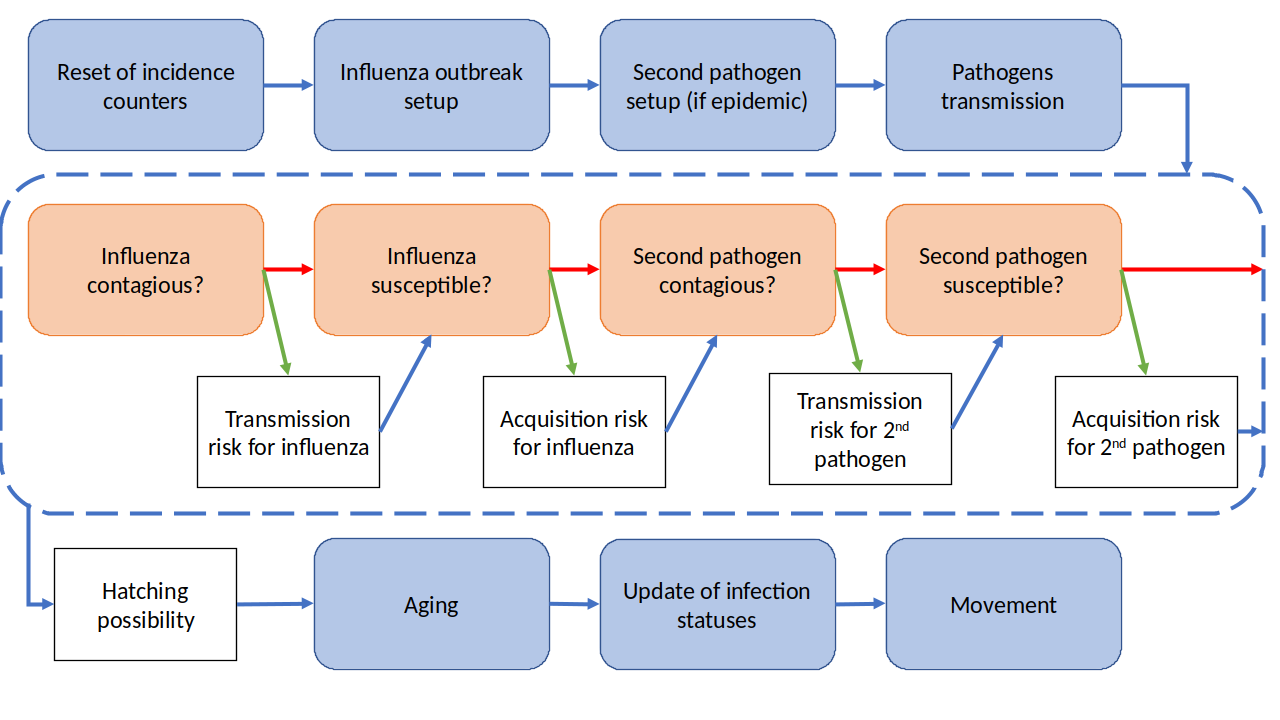
\includegraphics[width=\textwidth]{figures/analysis/workflow.png}
	\end{center}
}


\sframe{Interaction mechanisms}{
	\begin{table}
	\begin{center}
	\makegapedcells
	\begin{scriptsize}
	\begin{tabular}{|c|c|c|c|}
		\hline
		\textit{Risk} & \textit{acquisition} & \textit{transmission} & \textit{infection} \\
		\hline
		\diagbox{\thead{Influenza}}{\thead{Second\\pathogen}} & \thead{Susceptible} & \thead{Infected} & \thead{Colonised} \\
		\hline
		\multirow{2}{*}{\thead{Susceptible}} & $\beta$ & $\beta$ & $p$ \\
		& \textit{no interaction} & \textit{no interaction} & \textit{no interaction} \\
		\hline
		\multirow{3}{*}{\thead{Infected}} &  $\color{red}{\beta \times A}$ & $\color{red}{\beta \times \Theta}$ & $\color{red}{p \times \Pi}$ \\
		& \textit{acquisition} & \textit{transmission} & \textit{pathogénicité} \\
		& \textit{mechanism} & \textit{mechanism} & \textit{mechanism} \\
		\hline
	\end{tabular}
	\end{scriptsize}
	\end{center}
	\end{table}

	\visible<2>{
	\head{Interaction scenario}
	\begin{itemize}
		\item $A = \Theta = \Pi = 1 \rightarrow$ baseline scenario, no interaction
		\item $A \in [2 ; 50]$ ; $\Theta = \Pi = 1$
		\item $\Theta \in [2 ; 17]$ ; $A = \Pi = 1$
		\item $\Pi \in [5 ; 50]$ ; $A = \Theta = 1$
	\end{itemize}
	}
}



\subsection{Simulations du modèle}

\sframe{Simulated data}{
	\begin{columns}
	\begin{column}{.6\textwidth}
		\begin{center}
		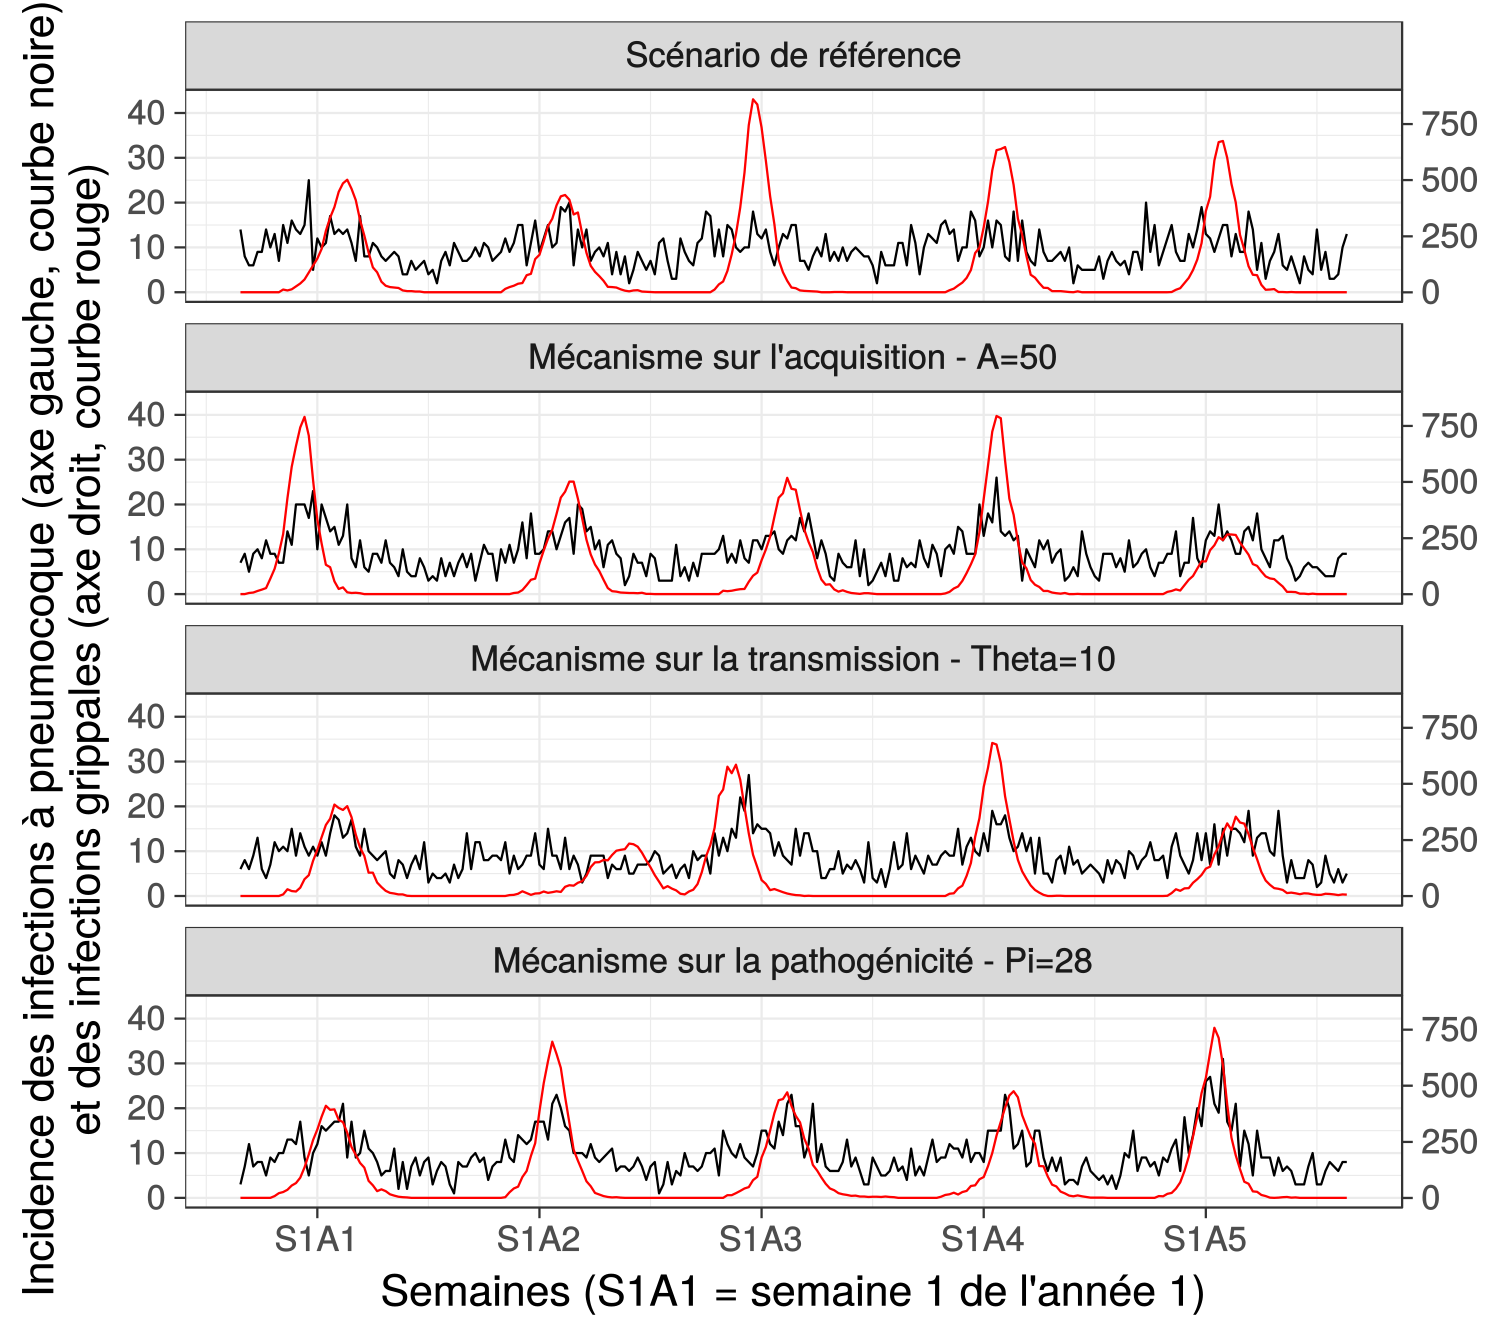
\includegraphics[width=\textwidth]{figures/model/incidences.png}
		\end{center}
	\end{column}
	\begin{column}{.47\textwidth}
		\head{Validation criteria}
		
		\begin{itemize}
			\item Influenza {\tiny \textit{Sentinelles}}
			\begin{itemize}
				\item Annual number of cases
				\item Epidemic onset
				\item Peak timing
				\item Epidemic duration
			\end{itemize}
			\medskip
			\item Pneumococcal infections
			\begin{itemize}
				\item Annual number of cases {\tiny \textit{Epibac}}
				\item Seasonality {\tiny \textit{Météo France}}
			\end{itemize}
		\end{itemize}
	\end{column}
	\end{columns}
}



%\subsection{Conclusion}
%
%\sframe{Conclusions}{
%	\begin{itemize}
%		\item Premier modèle individu-centré de co-circulation de la grippe en interaction avec un second pathogène
%		\begin{itemize}
%			\item dynamiques réalistes
%			\item pathogènes en interaction adaptables
%		\end{itemize}
%		\medskip
%		\visible<2->{
%		\item Plusieurs mécanismes d'interaction implémentés
%		\begin{itemize}
%			\item dynamiques différentes selon le mécanisme
%			\item possibilité d'ajout de mécanismes
%		\end{itemize}
%		}
%		\medskip
%		\visible<3->{
%		\item Étude de simulation
%		\begin{itemize}
%			\item suivi des cas d'infections à pneumocoque liés à l'interaction avec la grippe
%			\item effet limité de la grippe au niveau populationnel, même quand interaction forte au niveau individuel
%		\end{itemize}		
%		}
%	\end{itemize}
%}